\documentclass[11pt,a4paper]{article}

% DSA 8401 Applied Machine Learning Capstone Report
% Strathmore blue/red, Carlito typography, spacious layout and ruled footer.
\usepackage{iftex}
\ifXeTeX
  \usepackage{fontspec}
  \setmainfont{Carlito}
\else
  \usepackage[T1]{fontenc}
  \usepackage[sfdefault]{carlito}
\fi

\usepackage[a4paper,margin=1in,headheight=16pt,headsep=22pt,footskip=28pt]{geometry}
\usepackage{microtype}
\usepackage{setspace}
\setstretch{1.13}
\usepackage[parfill]{parskip}
\setlength{\parskip}{6pt}
\setlength{\parindent}{0pt}

\usepackage{graphicx}
% Figures live in reports/figures; these paths work whether the report is
% compiled from reports/final_report or from the repository root.
\graphicspath{{../figures/}{reports/figures/}{./}}
\usepackage{booktabs}
\usepackage{tabularx}
\usepackage{array}
\usepackage{float}
\usepackage{enumitem}
\usepackage{needspace}
\usepackage{titlesec}
\usepackage{xcolor}
\usepackage{fancyhdr}
\usepackage{caption}
\usepackage{hyperref}
\usepackage{xurl}
\usepackage[most]{tcolorbox}
\usepackage{tikz}

% Strathmore-inspired palette
\definecolor{StrathBlue}{HTML}{2A4591}
\definecolor{Ink}{HTML}{263238}
\definecolor{SoftBlue}{HTML}{F1F4FA}
\definecolor{Muted}{HTML}{667085}

\hypersetup{
  colorlinks=true,
  linkcolor=StrathBlue,
  urlcolor=StrathBlue,
  citecolor=StrathBlue,
  pdftitle={Predicting Traditional Bank Use Among Kenyan Adults},
  pdfauthor={Faith Makena Riungu}
}
\urlstyle{same}
\renewcommand{\arraystretch}{1.25}
\setlist{itemsep=3pt,topsep=4pt,leftmargin=*}
\setlist[enumerate]{label=\textcolor{StrathBlue}{\bfseries\arabic*.}}
\setlist[itemize]{label=\textcolor{StrathBlue}{\textbullet}}

% Section hierarchy
\definecolor{StrathGold}{HTML}{C5A044}

\titleformat{\section}
  {\Large\bfseries\color{StrathBlue}}
  {\thesection}{0.65em}{}
  [\vspace{3pt}{\color{StrathGold}\titlerule[1pt]}]
\titleformat{\subsection}
  {\large\bfseries\color{StrathBlue}}
  {\thesubsection}{0.65em}{}
\titleformat{\subsubsection}
  {\normalsize\bfseries\color{Ink}}
  {\thesubsubsection}{0.65em}{}
\titlespacing*{\section}{0pt}{20pt}{9pt}
\titlespacing*{\subsection}{0pt}{13pt}{5pt}
\titlespacing*{\subsubsection}{0pt}{10pt}{4pt}

% Header and footer
\pagestyle{fancy}
\fancyhf{}
\renewcommand{\headrulewidth}{0pt}
\renewcommand{\footrulewidth}{0.4pt}
\fancyfoot[L]{\textcolor{StrathBlue}{\textbf{\thepage}}\,|\,\textcolor{gray}{P a g e}}
\fancypagestyle{plain}{\fancyhf{}\renewcommand{\headrulewidth}{0pt}%
  \renewcommand{\footrulewidth}{0.4pt}%
  \fancyfoot[L]{\textcolor{StrathBlue}{\textbf{\thepage}}\,|\,\textcolor{gray}{P a g e}}}

% Tables and figures
\captionsetup{font=small,labelfont={bf,color=StrathBlue},textfont=it,skip=6pt}
\newcolumntype{L}{>{\raggedright\arraybackslash}X}
\newtcolorbox{summarybox}{
  enhanced,breakable,
  colback=SoftBlue,colframe=StrathBlue,
  boxrule=0.6pt,arc=2mm,
  left=3mm,right=3mm,top=2mm,bottom=2mm
}
\newcommand{\keyterm}[1]{\textcolor{StrathBlue}{\textbf{#1}}}

\begin{document}

% Title page styled to match the student's previous Strathmore assignment.
\hypersetup{pageanchor=false}
\begin{titlepage}
\thispagestyle{empty}
\centering
\vspace*{0.3in}

\includegraphics[width=1.45in]{Strathmore logo.png}\par
\vspace{0.35in}
{\fontsize{14}{17}\selectfont\color{StrathBlue}\bfseries STRATHMORE UNIVERSITY}\par\vspace{14pt}
{\fontsize{13}{16}\selectfont Master of Science in Data Science \& Analytics}\par\vspace{14pt}
{\fontsize{13}{16}\selectfont School of Computing and Engineering Sciences}\par\vspace{14pt}
DSA 8401: Applied Machine Learning in Data Science\par\vspace{18pt}
\textbf{Predicting Traditional Bank Use Among Kenyan Adults}\\[5pt]
A Machine Learning and Gender-Fairness Analysis\par\vspace{18pt}
Faith Makena Riungu-146570\par\vspace{12pt}
November 2026\par
\vfill
\end{titlepage}

\hypersetup{pageanchor=true}
\setcounter{page}{1}

\begin{summarybox}
\textbf{Abstract}\par

This project develops and evaluates machine-learning classifiers for predicting traditional bank use among Kenyan adults using the 2024 FinAccess Household Survey. It also examines whether prediction errors differ between women and men and evaluates whether changing the classification threshold can reduce observed disparities. The analysis uses survey weights, cluster-aware validation and a held-out test set. Gradient Boosting achieved the highest mean survey-weighted precision--recall area under the curve (PR-AUC) during model selection (0.712). On the held-out test set, its weighted PR-AUC was 0.753 and ROC-AUC was 0.871. At the conventional 0.50 threshold, recall was 51.9\% for women and 67.5\% for men, a difference of 15.6 percentage points. A common threshold of 0.320 reduced this gap to 9.1 percentage points and increased weighted F1, but also increased the false-positive rate. The findings demonstrate the value of evaluating predictive performance by gender and treating threshold adjustment as a trade-off rather than proof that a model is fair.
\end{summarybox}

\textcolor{StrathBlue}{\textbf{Keywords:}} financial inclusion; traditional bank use; machine learning; gender fairness; survey weights; Kenya.

\section{Introduction}

Financial inclusion is commonly discussed in terms of access to and use of formal financial services. However, aggregate inclusion statistics can conceal differences in how financial services are used across population groups. Predictive models may also perform differently for different groups, even when a sensitive attribute such as gender is excluded from the model inputs.

This project investigates whether respondent and household characteristics can predict traditional bank use among Kenyan adults and whether the resulting predictions exhibit gender-based performance differences. The project is predictive rather than causal: it does not estimate the effect of any characteristic or intervention on bank use.

\subsection{Problem statement and objectives}

The central problem is that a model with acceptable overall performance may identify actual bank users at different rates among women and men. This matters where model predictions could inform research, outreach or service planning. The project therefore has three objectives:
\begin{enumerate}[leftmargin=*]
  \item Develop and compare machine-learning models for predicting traditional bank use among Kenyan adults.
  \item Evaluate overall and gender-disaggregated predictive performance using survey-weighted metrics.
  \item Examine whether alternative classification thresholds can reduce the observed gender recall gap, while documenting the associated trade-offs.
\end{enumerate}

\section{Data and problem formulation}

\subsection{Data and study population}

The analysis uses the 2024 FinAccess Household Survey selected extract recorded in the project repository as 20,871 observations and 48 columns. The modelling population is restricted to respondents aged 18 years and above. This produces an adult sample of 19,750; 1,121 respondents below 18 years are excluded. The held-out test set contains 3,942 adults.

The project data manifest identifies the selected extract as \path{data/processed/finaccess_selected.csv}. Survey weights and cluster identifiers are retained for estimation and validation, respectively, but are not supplied as model predictors.

\subsection{Target variable}

The binary outcome is \texttt{target\_bank\_account}, derived from the FinAccess \texttt{Traditional\_bank} variable:
\begin{itemize}[leftmargin=*]
  \item Usage = 1;
  \item Non-usage = 0.
\end{itemize}

In the FinAccess 2024 data, \texttt{Traditional\_bank} records use of commercial bank products and excludes mobile-based bank products such as M-Shwari and KCB M-Pesa, so the outcome measures use of the traditional banking system rather than mobile-enabled banking.

\subsection{Predictors and sensitive attribute}

The primary model uses 35 predictors covering demographic, household, economic, digital and geographic characteristics. Examples include age, household size, income measures, education, wealth quintile, internet-use frequency, financial literacy, phone ownership, county, location type and livelihood category. Gender is retained for subgroup evaluation but excluded from the primary model inputs. Excluding gender does not guarantee that other predictors contain no gender-associated information.

\section{Methodology}

\subsection{Data preparation}

The project applies data cleaning and validation before modelling. Survey non-responses, refusals and ``Don't know'' values are not automatically interpreted as zero or ``No''. Numeric missing values are imputed using training-fold medians, with missingness indicators; missing categorical values are represented separately. Categorical predictors are one-hot encoded. Income amounts are converted to numeric values and log-transformed within the modelling pipeline. For 71 adults whose reported lowest monthly income exceeded their highest monthly income, both values were set to missing.

Learned preprocessing is fitted within each training fold to reduce information leakage from validation or test observations. Variables with unclear survey skip patterns or extensive missingness, identifiers, cluster identifiers, survey weights, gender and other financial-inclusion outcomes are excluded from the primary predictor set.

\subsection{Candidate models and justification}

Four approaches are compared:
\begin{itemize}[leftmargin=*]
  \item \textbf{Dummy classifier:} establishes a non-learning baseline.
  \item \textbf{Logistic Regression:} provides a relatively simple linear baseline.
  \item \textbf{Random Forest:} captures non-linear relationships and interactions through an ensemble of decision trees.
  \item \textbf{Gradient Boosting:} sequentially builds trees to improve predictive performance.
\end{itemize}
The models provide a comparison between a simple baseline, a linear classifier and two tree-ensemble approaches suited to structured survey data. Gradient Boosting was selected because it had the highest mean survey-weighted PR-AUC in cross-validation. Its advantage over Random Forest was modest, so the result is not interpreted as evidence of a large or statistically established superiority.

\subsection{Validation and survey weighting}

The project uses cluster-aware splitting so respondents from the same survey cluster are not distributed across training and evaluation partitions. Approximately 20\% of clusters are held out for final testing. Model selection uses nested group-aware cross-validation with five outer folds and three inner folds. The locked test set is not used to select the model or its operating threshold.

Survey weights are used in model fitting and weighted evaluation. Unweighted metrics are also retained to describe performance in the analysed sample. The primary model-selection metric is survey-weighted PR-AUC because the positive class is less common than the negative class and the analysis focuses on identifying bank users.

\subsection{Evaluation measures}

Overall performance is reported using PR-AUC, ROC-AUC, precision, recall (true-positive rate, TPR), F1 and Brier score. Fairness assessment compares women and men using TPR, false-negative rate (FNR), false-positive rate (FPR), selection rate, precision and calibration. The principal disparity measure is the male-minus-female TPR gap. Cluster-bootstrap confidence intervals are used for reported gender gaps. No single metric is treated as a complete definition of fairness.

\subsection{Threshold comparison}

The model produces predicted probabilities; a threshold converts these into predicted classes. Three rules are compared on the held-out test set: a common threshold of 0.50, a common threshold of 0.320 selected by maximising weighted F1 on training out-of-fold predictions, and gender-specific thresholds of 0.245 for women and 0.380 for men. The gender-specific thresholds are a comparison only; the final model package uses the common threshold of 0.320.

\subsection{Alternatives considered and excluded}

\begin{itemize}[leftmargin=*]
  \item \textbf{Stacking:} the three models were within one fold standard deviation of each other, leaving little for a meta-learner to gain, at the cost of extra complexity and harder explanations.
  \item \textbf{Deep learning:} the data are small and tabular; tree ensembles typically perform as well with less tuning and support exact TreeSHAP.
  \item \textbf{SMOTE and class weighting:} the imbalance is moderate (about 30\% positive); threshold adjustment handles it without distorting calibrated probabilities.
  \item \textbf{Fairness-constrained training:} post-processing was preferred because it keeps scores calibrated and makes the trade-off explicit; in-processing is left for future work.
  \item \textbf{Demographic parity:} bank use genuinely differs by gender, so equal selection rates would conflict with calibration; equal opportunity (equal TPR) was used instead.
\end{itemize}


\section{Results}

\subsection{Cross-validation model comparison}

Table~\ref{tab:cv} presents the mean survey-weighted PR-AUC across the outer cross-validation folds. Gradient Boosting recorded the highest mean score (0.712), followed by Random Forest (0.703) and Logistic Regression (0.694). The difference between Gradient Boosting and Random Forest was approximately 0.009, which is small relative to the fold-to-fold standard deviations. The model was selected on the pre-specified mean PR-AUC criterion, while recognising that the performance difference is modest.

\begin{table}[H]
\centering
\caption{Cross-validation model comparison}
\label{tab:cv}
\begin{tabular}{lcc}
\toprule
Model & Mean weighted PR-AUC & Standard deviation\\
\midrule
Dummy classifier & 0.286 & 0.006\\
Logistic Regression & 0.694 & 0.035\\
Random Forest & 0.703 & 0.034\\
\textbf{Gradient Boosting} & \textbf{0.712} & \textbf{0.029}\\
\bottomrule
\end{tabular}
\end{table}

\subsection{Held-out test performance}

On the 3,942-person test set, Gradient Boosting achieved a survey-weighted PR-AUC of 0.753, compared with a weighted chance baseline of 0.304. Its weighted ROC-AUC was 0.871, precision was 0.733, recall was 0.613, F1 was 0.668 and Brier score was 0.131 at the 0.50 threshold. The unweighted ROC-AUC was 0.872 and unweighted PR-AUC was 0.727. These results indicate useful ranking performance, but do not by themselves establish that the model is equally reliable across groups.

\begin{table}[H]
\centering
\caption{Overall held-out test performance at threshold 0.50}
\label{tab:test}
\begin{tabular}{lrr}
\toprule
Metric & Survey-weighted & Unweighted\\
\midrule
Base rate & 0.304 & 0.263\\
Precision & 0.733 & 0.718\\
Recall / TPR & 0.613 & 0.579\\
F1 & 0.668 & 0.641\\
PR-AUC & 0.753 & 0.727\\
ROC-AUC & 0.871 & 0.872\\
Brier score & 0.131 & 0.121\\
\bottomrule
\end{tabular}
\end{table}

\subsection{Gender-based performance}

At threshold 0.50, weighted recall was 0.519 for women and 0.675 for men. The male-minus-female TPR gap was 0.156, or 15.6 percentage points, with a 95\% confidence interval from 7.2 to 23.1 percentage points. The weighted FPR was also higher for men (0.135) than women (0.069), a gap of 6.6 percentage points (95\% CI: 3.3--9.9 percentage points). The weighted prevalence of bank use differed between women (0.234) and men (0.380), which is relevant when interpreting group metrics.

\begin{table}[H]
\centering
\caption{Gender-disaggregated weighted test metrics at threshold 0.50}
\label{tab:gender}
\begin{tabular}{lrr}
\toprule
Metric & Female & Male\\
\midrule
Test observations & 2,307 & 1,635\\
Base rate & 0.234 & 0.380\\
Selection rate & 0.174 & 0.340\\
Precision & 0.697 & 0.753\\
Recall / TPR & 0.519 & 0.675\\
FNR & 0.481 & 0.325\\
FPR & 0.069 & 0.135\\
PR-AUC & 0.707 & 0.782\\
ROC-AUC & 0.880 & 0.853\\
\bottomrule
\end{tabular}
\end{table}

The segment results also show variation by location. At the 0.50 threshold, recall was 0.493 for rural women and 0.558 for rural men. In urban areas, recall was 0.536 for women and 0.742 for men. These subgroup results suggest that an aggregate gender comparison can conceal further variation across location.

\subsection{Gender information in other predictors}

Gender is excluded from the model inputs, but other predictors may still carry gender information. To measure this, a classifier with the same architecture and hyperparameters as the final model was trained to predict respondent gender from the 35 predictors, using the training clusters only, and evaluated on the held-out test set. The predictors identified gender with a weighted ROC-AUC of 0.906. Removing relationship to household head reduced this to 0.851, and removing all four household-role variables (relationship to household head, marital status, and the two household spending-decision variables) reduced it to 0.772. Relationship to household head was the strongest single predictor of gender (ROC-AUC 0.756). Excluding gender from the inputs therefore does not make the model gender-blind.

\subsection{Calibration}

The predicted probabilities were well calibrated overall: the weighted expected calibration error (ECE) was 0.019 on the test set. Calibration was slightly weaker for men (ECE 0.038) than for women (ECE 0.027); the mean predicted probability for men was 0.359 against an observed bank-use rate of 0.380, a small under-prediction. Because the model is reasonably calibrated within each gender, no recalibration step was applied. Calibration within groups is also why demographic parity was not adopted as the fairness target: with bank use genuinely higher among men (0.380) than women (0.234), equal selection rates would require deliberately miscalibrated predictions.

\begin{figure}[H]
\centering
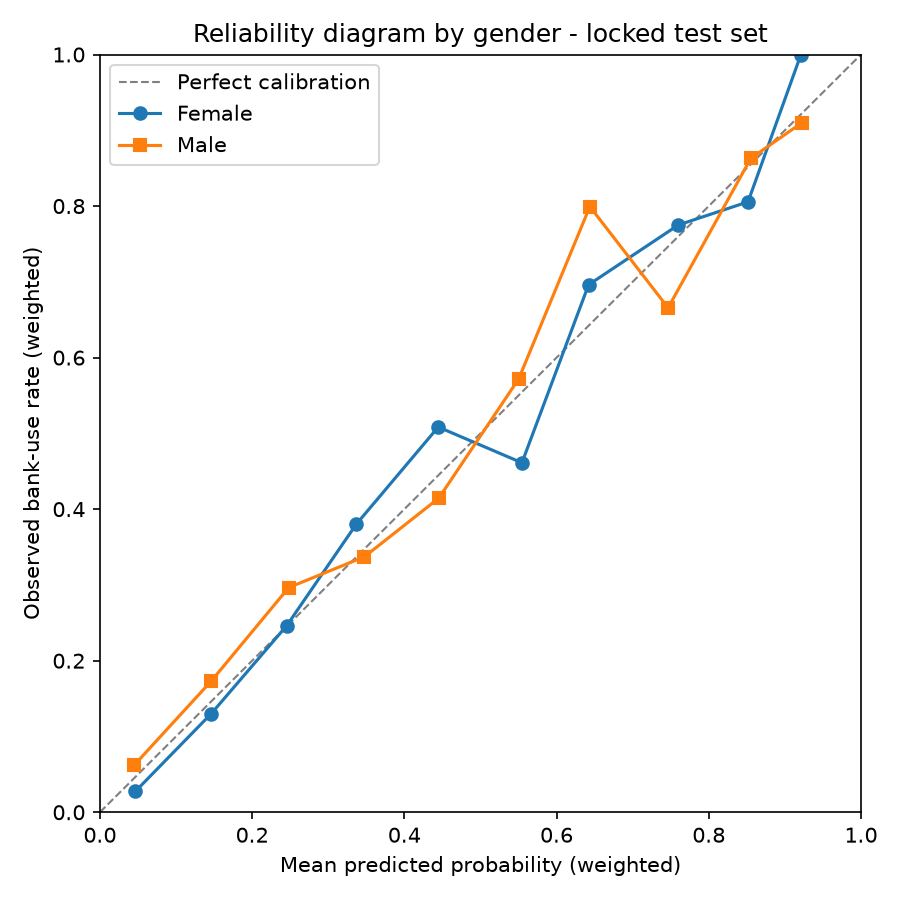
\includegraphics[width=0.55\textwidth]{calibration_by_gender.png}
\caption{Reliability diagram by gender on the held-out test set. Points close to the diagonal indicate well-calibrated predicted probabilities.}
\label{fig:calibration}
\end{figure}

\subsection{Threshold mitigation and trade-offs}

Table~\ref{tab:threshold} compares the three threshold rules. Moving from 0.50 to the common 0.320 threshold increased weighted F1 from 0.668 to 0.690 and reduced the TPR gap from 15.6 to 9.1 percentage points. However, the weighted FPR increased from 0.097 to 0.191. The confidence interval for the remaining TPR gap at 0.320 was 2.2--15.5 percentage points, so the observed disparity was not eliminated.

Gender-specific thresholds reduced the point-estimate TPR gap to -5.2 percentage points, with a confidence interval spanning -13.1 to 2.5 percentage points. This approach uses gender at decision time and is not the rule adopted in the final model package. It is reported to illustrate the potential fairness-performance trade-off, not as an automatic deployment recommendation.

\begin{table}[H]
\centering
\caption{Threshold comparison on the held-out test set}
\label{tab:threshold}
\small
\begin{tabular}{lrrrr}
\toprule
Threshold rule & Weighted F1 & Female TPR & Male TPR & TPR gap (M--F)\\
\midrule
Common 0.50 & 0.668 & 0.519 & 0.675 & 0.156\\
Common 0.320 & 0.690 & 0.703 & 0.794 & 0.091\\
Gender-specific (0.245 / 0.380) & 0.691 & 0.806 & 0.754 & -0.052\\
\bottomrule
\end{tabular}
\end{table}

\begin{figure}[H]
\centering
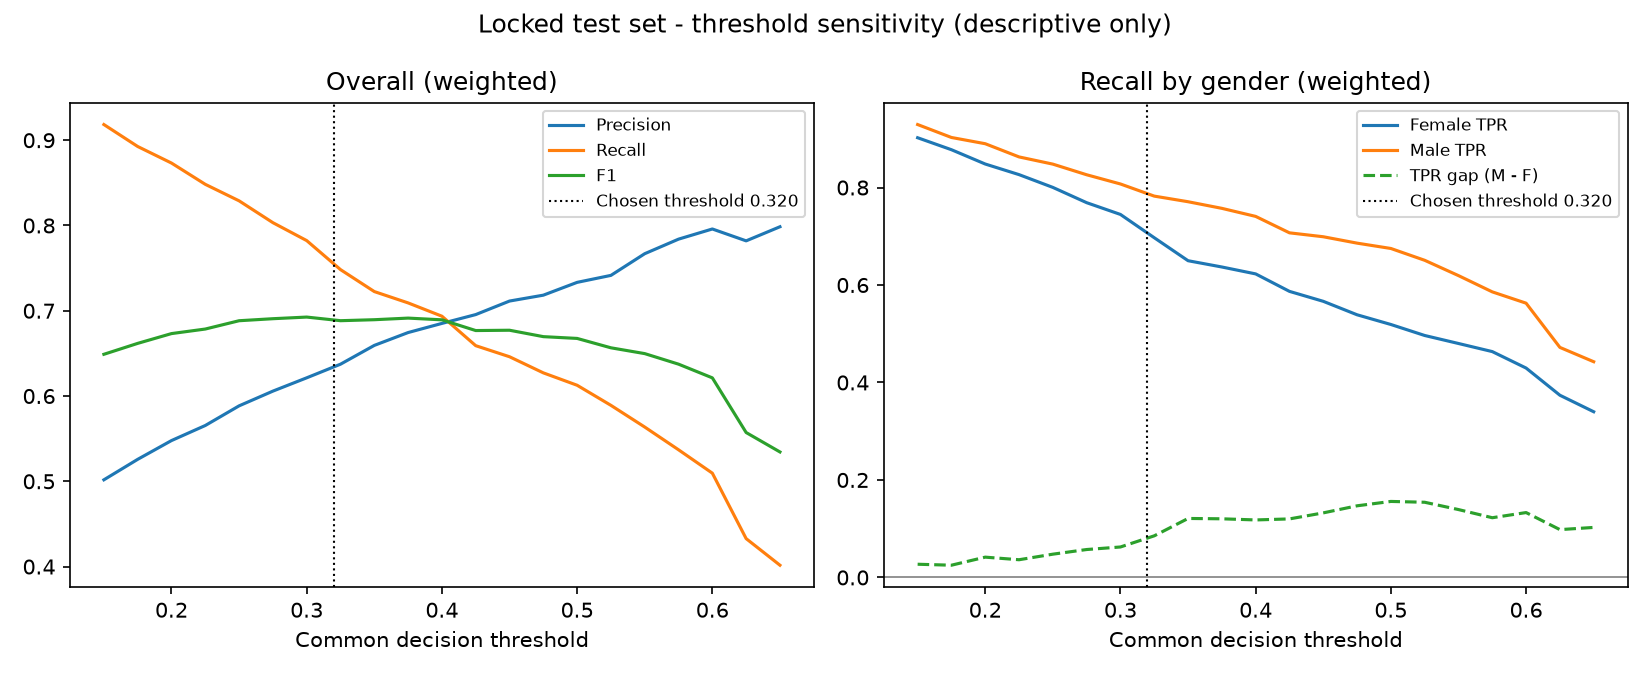
\includegraphics[width=0.82\textwidth]{threshold_sweep_test.png}
\caption{Test-set threshold sweep. This figure is descriptive; threshold selection was performed using training out-of-fold predictions.}
\label{fig:threshold}
\end{figure}

\subsection{Model interpretation}

TreeSHAP was used to examine the contribution of predictors to the fitted Gradient Boosting model. The highest weighted mean absolute SHAP values were observed for age (0.375), internet-use frequency (0.298), education level (0.267), income in the last month (0.265), possession of an identity document (0.258) and highest monthly income (0.256). These values describe the model's reliance on features when producing predictions. They do not establish that the features cause traditional bank use.

\begin{figure}[H]
\centering
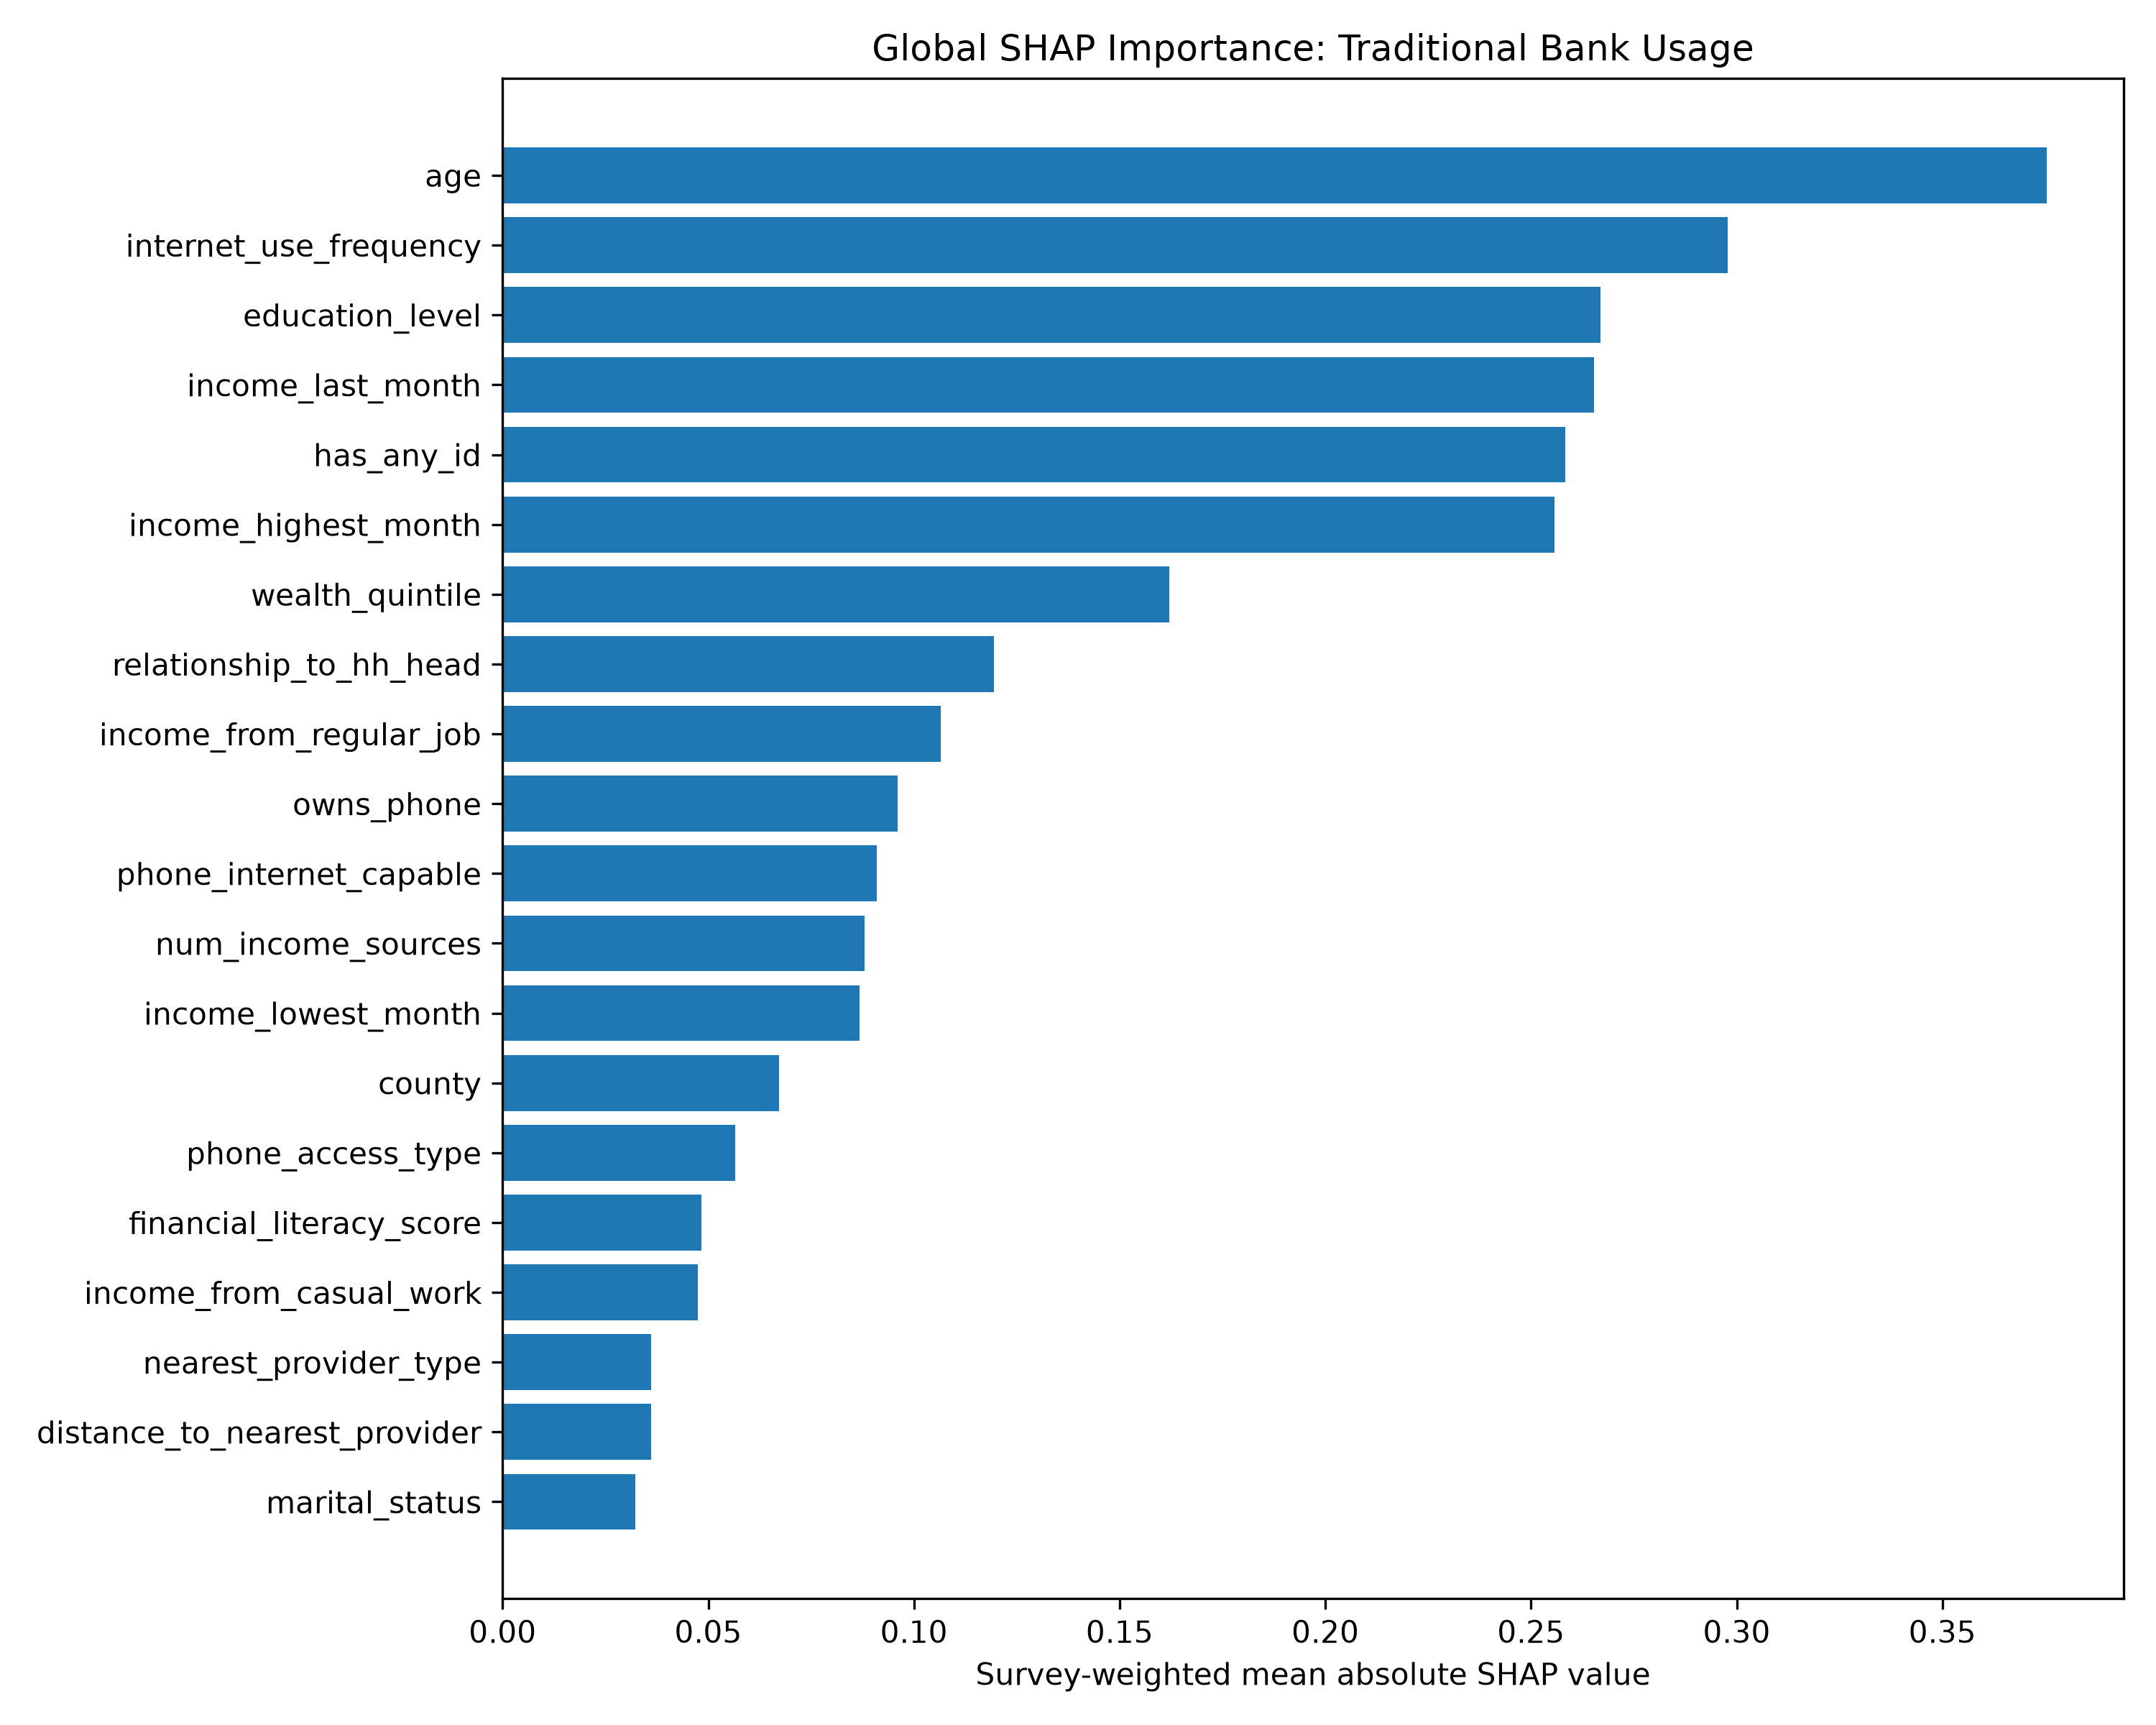
\includegraphics[width=0.82\textwidth]{shap_global_importance.png}
\caption{Global SHAP feature importance for the fitted model.}
\label{fig:shap}
\end{figure}

Comparing SHAP values by gender helps explain the recall gap. The same predictors matter for women and men, but several push predictions in opposite directions. Income in the last month lowered women's scores on average (mean SHAP $-0.052$) and raised men's ($+0.112$); highest monthly income followed the same pattern ($-0.033$ and $+0.113$). Relationship to household head also lowered women's scores ($-0.073$) and raised men's ($+0.076$). Lower personal income and household position therefore hold down women's predicted probabilities, so more women who do use banks fall below the threshold. At the deployed 0.320 threshold, the held-out test set contains 284 false negatives (bank users predicted as non-users) and 479 false positives.

\section{Deployment artefact}

The trained model is packaged with its decision threshold (0.320), input schema and metadata, and served through a FastAPI service with prediction, batch-prediction, health and metadata endpoints. Invalid inputs are rejected (HTTP 422), gender is not an accepted input, and each prediction returns its probability, decision and the three largest SHAP contributions as reason codes. The service runs in a Docker container (non-root, read-only, with a health check) that reproduces the offline model's predictions exactly, and 36 automated tests cover the pipeline, model package and API. This is a reproducible demonstration, not a system ready for individual financial-service decisions.

\section{Limitations}

The findings should be interpreted in light of the following limitations:
\begin{enumerate}[leftmargin=*]
  \item \textbf{Single survey round:} the analysis uses one cross-sectional survey round. Performance and relationships may change in later years or under different economic conditions.
  \item \textbf{Predictive, not causal:} the models identify patterns associated with traditional bank use and cannot establish causal effects.
  \item \textbf{Residual proxy information:} excluding gender from model inputs does not remove gender information. The other predictors identify respondent gender with a test ROC-AUC of 0.906, mainly through household-role variables.
  \item \textbf{Metric trade-offs:} reducing the TPR gap through threshold adjustment increased the false-positive rate. Fairness cannot be summarised by one metric.
  \item \textbf{Subgroup uncertainty:} estimates for smaller gender-by-location groups are less precise and should be interpreted cautiously.
  \item \textbf{External validation:} the repository reports a cluster-held-out test evaluation, but does not establish performance on an independent survey or future population.
\end{enumerate}


\section{Conclusion and recommendations}

\subsection{Conclusion}

This project shows that traditional bank use among Kenyan adults can be predicted usefully from survey characteristics, but that overall performance alone does not show whether a model works equally well for everyone.

Gradient Boosting was the strongest of the three learning models in cross-validation (weighted PR-AUC 0.712), though its lead over Random Forest was small. On the held-out test set it achieved a weighted PR-AUC of 0.753 and ROC-AUC of 0.871.

The model was markedly less reliable for women. At the 0.50 threshold, it correctly identified 51.9\% of women who use banks, compared with 67.5\% of men: a gap of 15.6 percentage points. Gender was not a model input, yet the other predictors identified gender with a ROC-AUC of 0.906, so excluding gender did not prevent the disparity.

Lowering the common threshold to 0.320 narrowed the gap to 9.1 percentage points and raised weighted F1 from 0.668 to 0.690, but nearly doubled the false-positive rate, from 9.7\% to 19.1\%. Threshold adjustment reduced the disparity without removing it.

Predictive performance and fairness must therefore be evaluated together. A model can perform well overall while serving some groups less well, and gender-disaggregated evaluation is needed to see this.

\subsection{Recommendations}

\begin{enumerate}
  \item \textbf{Report performance by group.} Evaluate financial-inclusion models separately for women and men, and where samples allow, by location, using recall, FNR, FPR, precision and selection rate, not aggregate AUC alone.
  \item \textbf{Treat the threshold as a policy choice.} The 0.320 threshold balanced F1 and the recall gap better than 0.50, at the cost of more false positives. Any use of the model should state why a threshold was chosen and weigh the costs of both error types.
  \item \textbf{Validate before operational use.} Test the model on later FinAccess rounds and independent data to confirm that its performance and gender gaps hold over time.
  \item \textbf{Investigate the drivers of the gap.} SHAP points to income and household position as sources of lower scores for women; these should be examined further, as model explanations rather than causes.
  \item \textbf{Use the model for analysis, not eligibility.} The model is a research artefact and should not determine individual access to financial services without independent validation, governance and fairness monitoring.
\end{enumerate}

\subsection{Areas for future research}

Future research could extend this work by incorporating additional
FinAccess survey rounds to examine changes in traditional bank use
over time. Further investigation could also explore intersectional
fairness across gender, county and rural urban residence, subject
to adequate subgroup sample sizes. Finally, alternative fairness
interventions, including fairness-constrained (in-processing) training, and calibration approaches could be compared to
determine whether disparities can be reduced without introducing
unacceptable increases in classification errors.


\end{document}